\documentclass[abstract=true]{scrartcl}
\usepackage{amsthm,amsmath,amssymb}
\usepackage[utf8]{inputenc}
\usepackage{tikz}
\usetikzlibrary{arrows.meta,hobby,calc}
\usepackage{tikz}
\usepackage{pgfplots}
\pgfplotsset{compat=1.15}
\usepackage{pgfmath}
\usetikzlibrary{arrows.meta}
\usetikzlibrary{decorations.markings}
\usetikzlibrary{shapes.geometric}
\usetikzlibrary{calc}
\usetikzlibrary{fillbetween}

\begin{document}

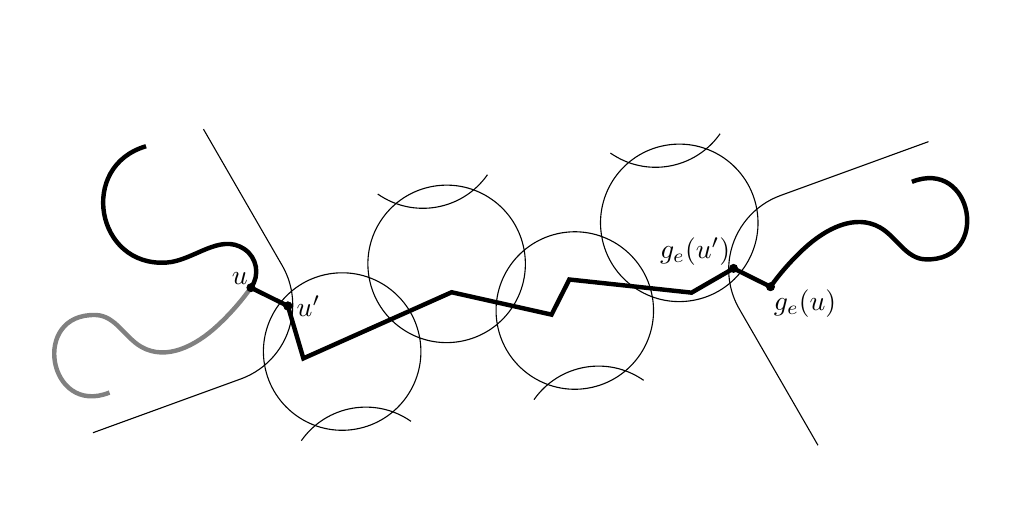
\begin{tikzpicture}[use Hobby shortcut,vertex/.style={inner sep=1pt,circle,draw,fill},rotate=10]
    \draw (0,0) 
    circle(1cm)
    ++(0:1cm)
    ++(60:1cm)
    circle(1cm)
    ++(0:1cm)
    ++(-60:1cm)
    circle(1cm)
    ++(0:1cm)
    ++(60:1cm)
    circle(1cm);

    %top arcs
    \draw (0,0)
    ++(0:1cm)
    ++(60:1cm)
    ++(60:1cm)
    ++(120:1cm)
    ++(-45:1) arc (-45:-135:1) ++(-135:-1)
    ++(0:1cm)
    ++(60:1cm)
    ++(0:1cm)
    ++(-60:1cm)
    ++(-45:1) arc (-45:-135:1) ++(-135:-1);

    %bottom arcs
    \draw (0,0)
    ++(-60:1cm)
    ++(-120:1cm)
    ++(45:1) arc (45:135:1) ++(135:-1)
    ++(0:1cm)
    ++(60:1cm)
    ++(0:1cm)
    ++(-60:1cm)
    ++(45:1) arc (45:135:1) ++(135:-1);

    \draw (0,0)
    ++(180:1cm)
    ++(120:1cm)
    ++(-80:1)
    ++(190:2)
    -- ++(10:2)
    arc (-80:20:1)
    -- ++(110:2);

    \draw (0,0)
    ++(0:3cm)
    ++(60:2cm)
    ++(-60:1cm)

    ++(180:-1cm)
    ++(120:-1cm)
    ++(-80:-1)
    ++(190:-2)
    -- ++(10:-2)
    arc (-80:20:-1)
    -- ++(110:-2);

    \draw[ultra thick]
    (-2,3)..(-2,1.5)..(-1,1.5)..(-1,1);
    \draw[gray, ultra thick]
    (-1,1)..(-1.5,0.6)..(-2.5,0.5)..(-3,1)..(-3,0);


    \draw[ultra thick]
    (-1,1)
    --(130:.9) 
    --(-.5,0)
    --(1.5,.5)
    --(2.7,0)
    --(3,.4)
    --++($(0,-.4) + (0:1) + (60:1) + (90:-.9)$)
    --++($(90:.9) + (-50:.9)$)
    --++($(130:.9) -(-1,1)$);
    \begin{scope}[shift = ($(0:1)+(60:1)$), xshift=3cm,rotate=180]
    \draw[ultra thick]
    (-1,1)..(-1.5,0.6)..(-2.5,0.5)..(-3,1)..(-3,0);
    \node[vertex] at (-1,1){};
    \node[inner sep = 1pt, anchor=north west] at (-1,1){$g_e(u)$};
    \node[inner sep = 1pt, anchor=south east] at (130:.9){$g_e(u')$};
    \node[vertex] at (130:.9) {};
    \end{scope}

    \node[vertex] at (-1,1){};
    \node[inner sep = 1pt, anchor=south east] at (-1,1){$u$};
    \node[vertex] at (130:.9) {};
    \node[inner sep =3pt,anchor=west] at (130:.9){$u'$};
    \node[vertex] at (130:.9) {};
\end{tikzpicture}

\end{document}